\section{Схема установки}

\begin{figure}[h]
	\begin{center}
		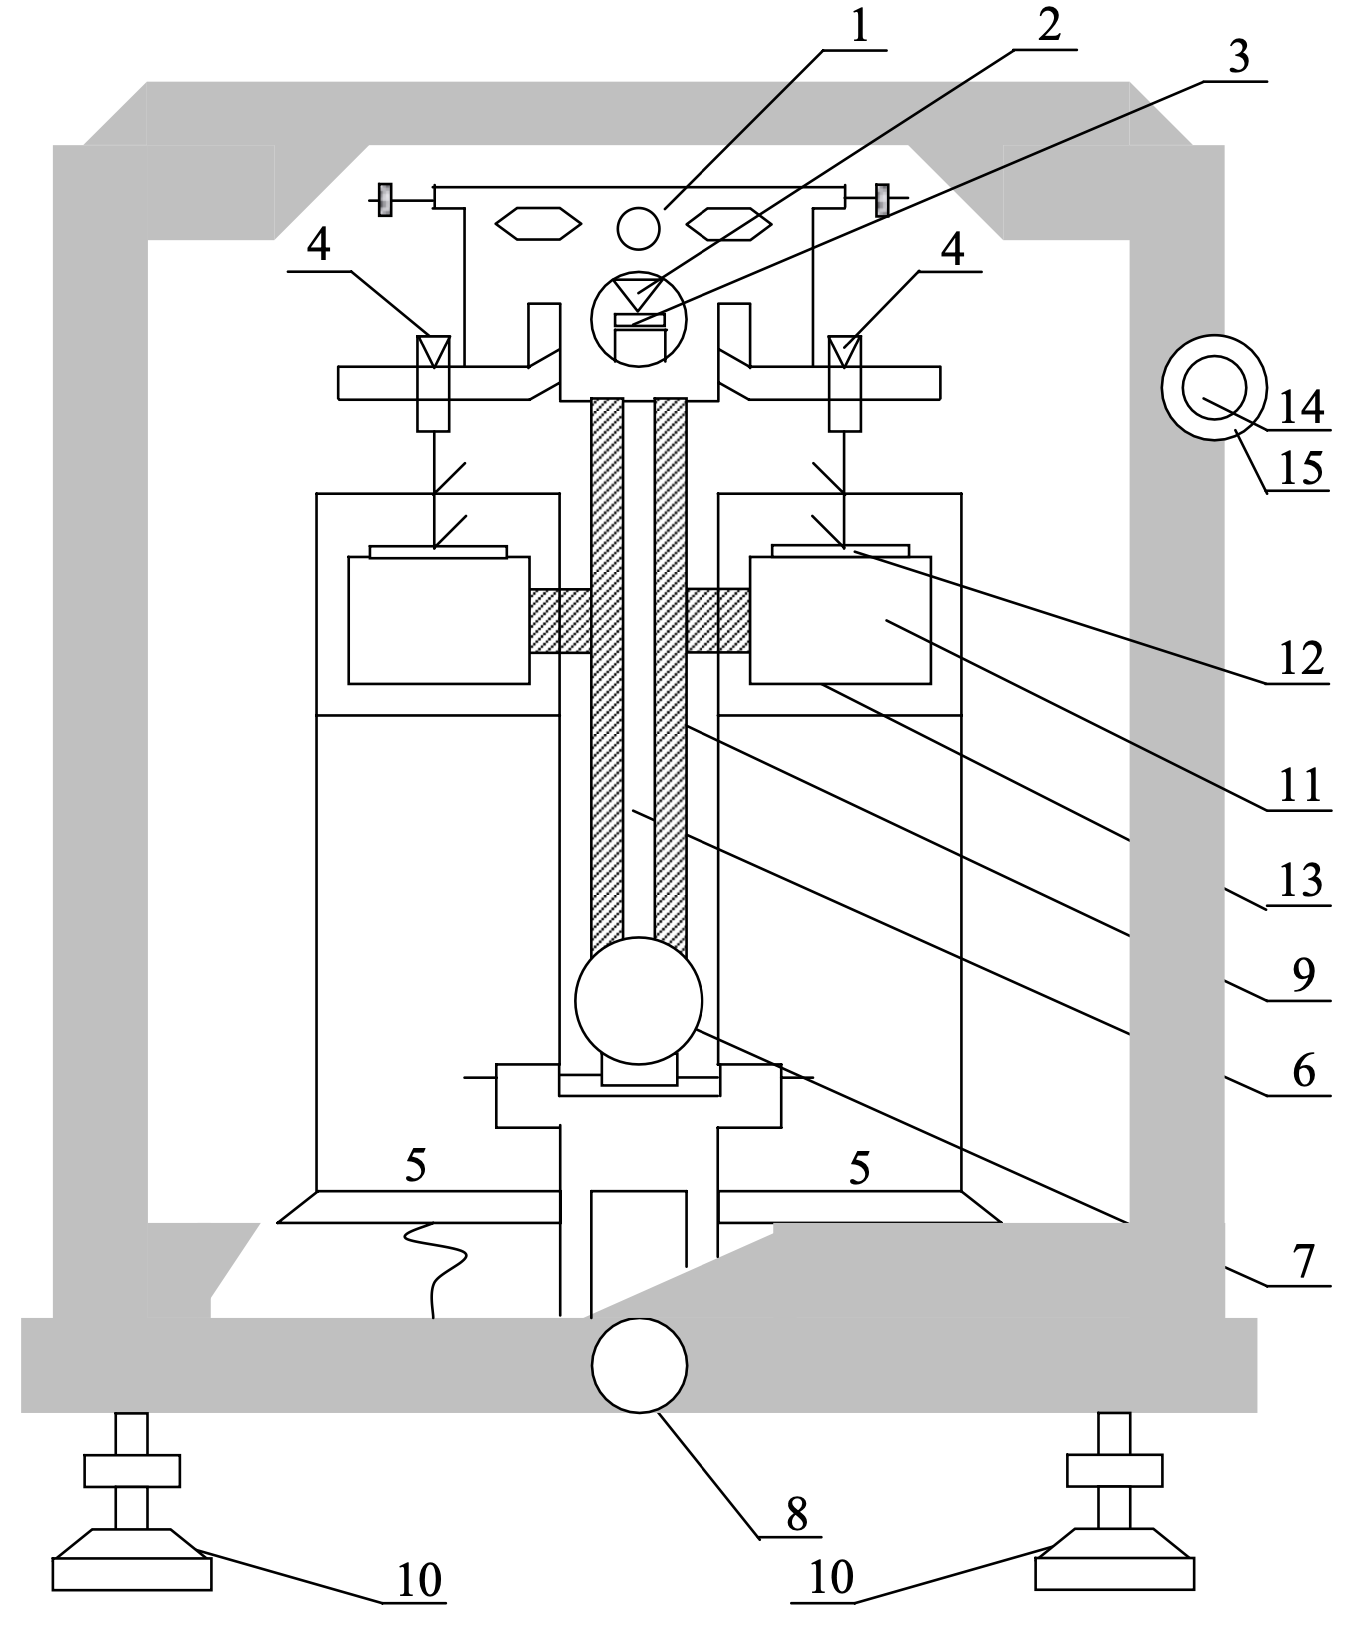
\includegraphics[width=0.7\textwidth]{pictures/PictureOne}
		\caption{Аналитические весы}\label{PicOne}
	\end{center}
\end{figure}

На рисунке~\ref{PicOne} изображены аналитические весы. Цифрой 1 обозначено коромысло, которое опирается призмой 2 на подошку 3. На призмах 4 подвешены чашки 5. Стрелкой 6 и шкалой 7 отмечается положение коромысла. Установка весов в горизонтальном положении осуществляется путём вращения ножек 10. Арретировка весов достигается поворотом ручки 8. При этом подушка опускается и коромысло ложится на колонку 9. Весы снабжены воздушным демпфером $11\div12$, наружная чашка которого прикреплена штангой 13 к колонке. Наложение гирь на коромысло осуществляется вращением малого и большого лимбов $14\div15$.